\documentclass{article}


\usepackage{circuitikz} %Für die Schaltpläne
\usepackage[T1]{fontenc}
\usepackage[utf8]{inputenc}
\usepackage{amsmath}
\usepackage{amssymb}
\usepackage{fancyhdr}
\usepackage{graphicx}
\usepackage{hyperref}
\usepackage{subcaption}
\usepackage{tikz}
\usepackage{../assets/scripts/tex/color-env}
\usepackage[ngerman]{babel}



    \usetikzlibrary{arrows}
    \usetikzlibrary{arrows.meta,topaths}
    \usetikzlibrary{bending}
    \usetikzlibrary{calc}
\title{Elektrotechnik 1 Praktikum 1}


\usepackage[
  includehead,
  headheight = 17mm,
  footskip = \dimexpr\headsep+\ht\strutbox\relax,
  tmargin = 0mm,
  bmargin = \dimexpr17mm+2\ht\strutbox\relax,
]{geometry}

\usepackage{anyfontsize}

\usepackage{xcolor}

\definecolor{DarkGreenBlue}{HTML}{264653}
\definecolor{LightGreenBlue}{HTML}{2A9D8F}
\definecolor{LightOrange}{HTML}{E9C46A}
\definecolor{DarkOrange}{HTML}{F4A261}
\definecolor{RedOrange}{HTML}{E76F51}
\definecolor{BrightRed}{HTML}{D62828}
\definecolor{DeepBlue}{HTML}{003049}



\pagestyle{fancy}
\fancyhead[L]{\leftmark}
\fancyhead[R]{}
\fancyfoot[L]{}
\fancyfoot[C]{\thepage}
\fancyfoot[R]{
\includegraphics[scale=0.2]{../assets/images/haw.jpg}}
\renewcommand\headrulewidth{0.5pt}


\begin{document}



\begin{tikzpicture}[overlay,remember picture]
  \thispagestyle{empty}
  \fill[black!2] (current page.south west) rectangle (current page.north east);

  \begin{scope}[transform canvas ={rotate around ={45:($(current page.north west)+(-.5,-6)$)}}]

    \shade[rounded corners=18pt, left color=DarkGreenBlue, right color=LightGreenBlue] ($(current page.north west)+(-.5,-6)$) rectangle ++(9,1.5);

  \end{scope}

  \begin{scope}[transform canvas ={rotate around ={45:($(current page.north west)+(.5,-10)$)}}]

    \shade[rounded corners=18pt, left color=LightOrange,right color=DarkOrange] ($(current page.north west)+(0.5,-10)$) rectangle ++(15,1.5);

  \end{scope}

  \begin{scope}[transform canvas ={rotate around ={45:($(current page.north west)+(0.5,-10)$)}}]

    \shade[rounded corners=8pt, right color=DarkOrange, left color=LightOrange] ($(current page.north west)+(1.5,-9.55)$) rectangle ++(7,.6);

  \end{scope}

  \begin{scope}[transform canvas ={rotate around ={45:($(current page.north)+(-1.5,-3)$)}}]

    \shade[rounded corners=12pt, left color=DeepBlue!80, right color=DeepBlue!60] ($(current page.north)+(-1.5,-3)$) rectangle ++(9,0.8);

  \end{scope}

  \begin{scope}[transform canvas ={rotate around ={45:($(current page.north)+(-3,-8)$)}}]

    \shade[rounded corners=28pt, left color=BrightRed, right color=BrightRed!80] ($(current page.north)+(-3,-8)$) rectangle ++(15,1.8);

  \end{scope}

  \begin{scope}[transform canvas ={rotate around ={45:($(current page.north west)+(4,-15.5)$)}}]

    \shade[rounded corners=25pt, left color=RedOrange, right color=DarkOrange] ($(current page.north west)+(4,-15.5)$) rectangle ++(30,1.8);

  \end{scope}

  \begin{scope}[transform canvas ={rotate around ={45:($(current page.north west)+(13,-10)$)}},]

    \shade[rounded corners=22pt, left color=DeepBlue,right color=DarkGreenBlue] ($(current page.north west)+(13,-10)$) rectangle ++(15,1.5);

  \end{scope}

  \begin{scope}[transform canvas ={rotate around ={45:($(current page.north west)+(18,-8)$)}},]

    \shade[rounded corners=8pt, left color=DarkOrange] ($(current page.north west)+(18,-8)$) rectangle ++(15,0.6);

  \end{scope}

  \begin{scope}[transform canvas ={rotate around ={45:($(current page.north west)+(19,-5.65)$)}},]

    \shade[rounded corners=12pt, left color=RedOrange] ($(current page.north west)+(19,-5.65)$) rectangle ++(15,0.8);

  \end{scope}

  \begin{scope}[transform canvas ={rotate around ={45:($(current page.north west)+(20,-9)$)}}]

    \shade[rounded corners=20pt, left color=BrightRed, right color=BrightRed!80] ($(current page.north west)+(20,-9)$) rectangle ++(14,1.2);

  \end{scope}

  \draw[ultra thick,gray] ($(current page.center)+(5,2)$) -- ++(0,-3cm) node[midway,left=0.25cm,text width=5cm,align=right,black!75]{{\fontsize{25}{30} \selectfont \bf Elektronik 2\\[10pt] Praktikum 1}} node[midway,right=0.25cm,text width=6cm,align=left,orange]{{\fontsize{70}{86} \selectfont 2021}};

  \node at ($(current page.center)+(0,-4)$) {{\fontsize{60}{72} \selectfont Differenzverstärker}};

  \node[text width=8cm,align=center] at ($(current page.center)+(0,-6.5)$) {{\fontsize{16}{20} \selectfont \textcolor{orange}{ \bf \today}} \\[3pt] Florian Tietjen\\[3pt] Eric Antosch};

\end{tikzpicture}
\newpage
\thispagestyle{empty}

\tableofcontents


\newpage


\section{Grundschaltung eines Differenzverstärkers}
\begin{task}
  TBei dieser Aufgabe soll die Grundschaltung eines Differenzverstärkers mit zwei BC546B-Transistoren mit beiden Basen an GND beschrieben werden.
\end{task}

\begin{figure}[h]
  \centering
  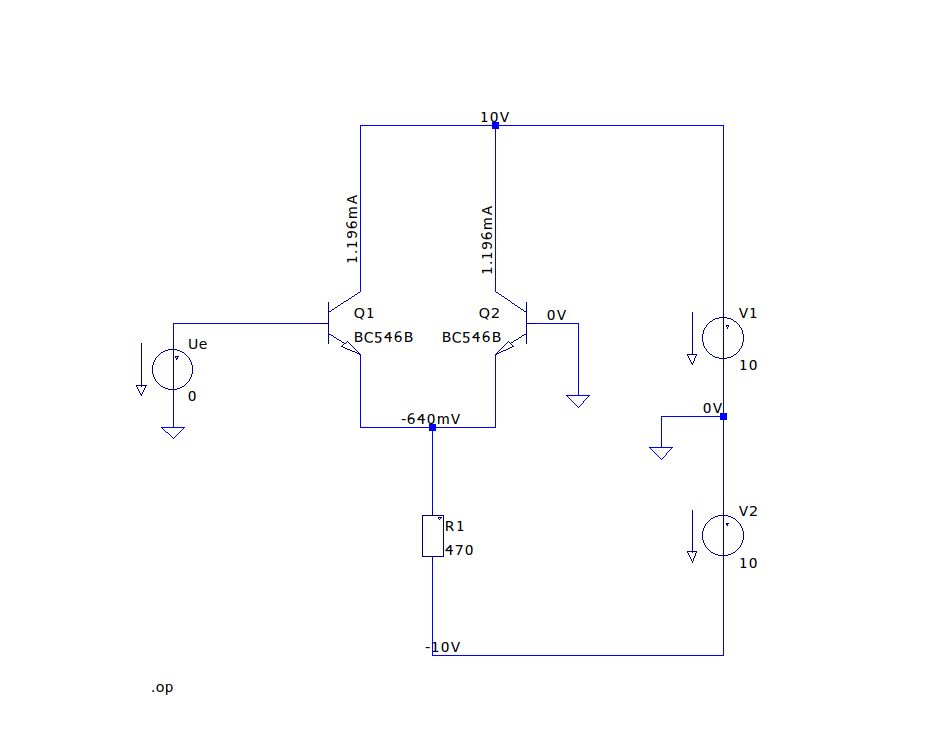
\includegraphics[scale=0.5]{../assets/images/EL2P1/DeepinScreenshot_select-area_20210417230640.png}
  \caption{Grundschaltung eines Differenzverstärkers}
  \label{fig:schalt1}
\end{figure}

\subsection{Dimensionierung des $R_E$-Widerstands}
\label{sec:RE}

Wir wollen nun zunächst unseren $R_E$-Widerstand mithilfe der gegebenen Formeln berechnen:
\begin{equation}
 R_E = \frac{U_B-U_{BE}}{2\cdot I_C} 
\end{equation}

Wir erhalten mit dem Einsetzen der Werte für $I_C = 1mA$, $U_B = 0V$ und $U_{BE} = 0,7V$ ungefähr
einen Widerstandswert von $R_E = 350\Omega$. Da unser Widerstand $R_E$ aus der E12-Reihe sein soll, 
wählen wir mit $470\Omega$ den passenden Widerstandswert.
\newpage

\section{Differenzverstärkung}

\begin{task}
  TIn dieser Aufgabe wollen wir die Differenzverstärkung unserer Grundschaltung ermitteln, indem wir den linken Transistor nun von einer Spannungsquelle
  ansteuern lassen.
\end{task}

\begin{figure}[h]
  \centering
  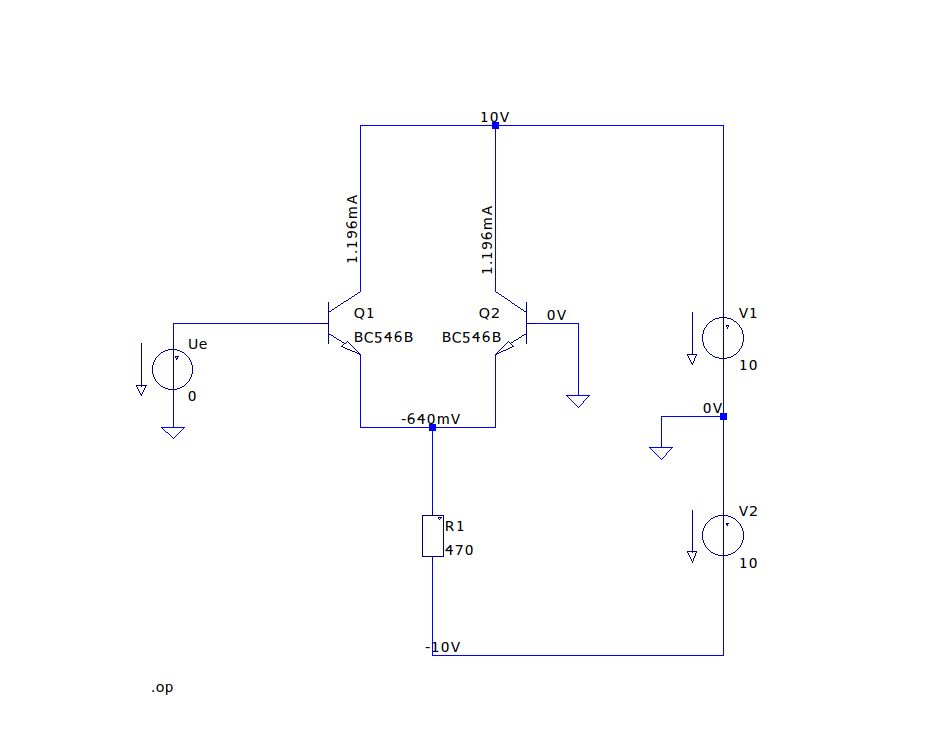
\includegraphics[scale=0.5]{../assets/images/EL2P1/DeepinScreenshot_select-area_20210417230640.png}
  \caption{Versuchsaufbau}
  \label{fig:schalt2}
\end{figure}

Wir nutzen nun die DC-Sweep-Analyse von LTSpice um die Spannung der Ue-Quelle linear von $-0,5V$ bis $0,5V$
wachsen zu lassen. Aus der Vorlesung kennen wir die Bedeutung von $U_d$, welches die Differenz der
Potentiale an den Basen der beiden Transistoren darstellt. 

\begin{equation}
  Placeholder
\end{equation}

Tragen wir nun die Ströme durch die beiden Transistoren gegen die Differenzspannung $U_d$ ab, so
entsteht folgendes Bild:

\begin{figure}[h]
  \centering
  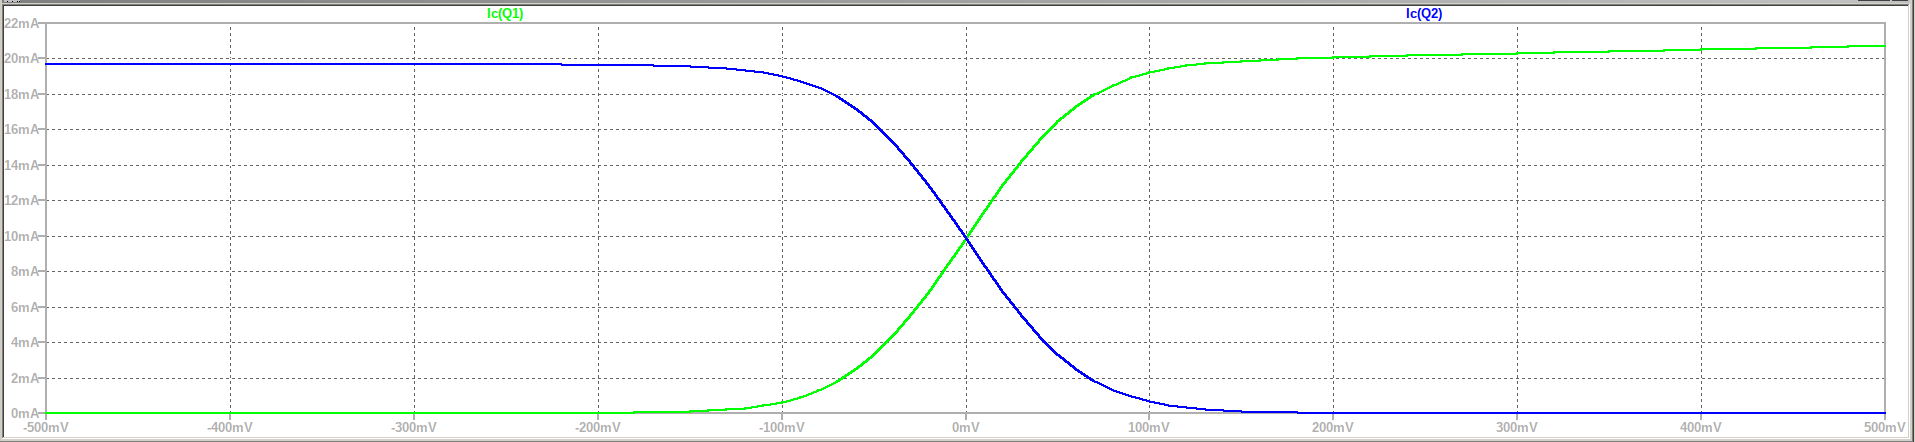
\includegraphics[scale=0.3]{../assets/images/EL2P1/DeepinScreenshot_select-area_20210417230438.png}
  \caption{Darstellung der Kollektorströme gegen die Differenzspannung $U_d$}
  \label{fig:diag1}
\end{figure}

Wir erkennen sowohl eine ziemlich genaue Übereinstimmung der Diagramme aus der Vorlesung als auch aus den
Praktikumsaufgaben.
Bei einer Differenzspannung von $U_d = 0V$ erhalten wir zudem unsere $I_C = 1 mA$, die wir in Aufgabe 1 bereits
verwendet haben. 
\newpage

\section{Wechselspannungsansteuerung}

\begin{task}
  TBei diesem Versuch werden nun zunächst nur der linke, dann beide Transistoren mit einer Wechselspannung
  angesteuert.
\end{task}

\begin{figure}[h]
  \centering
  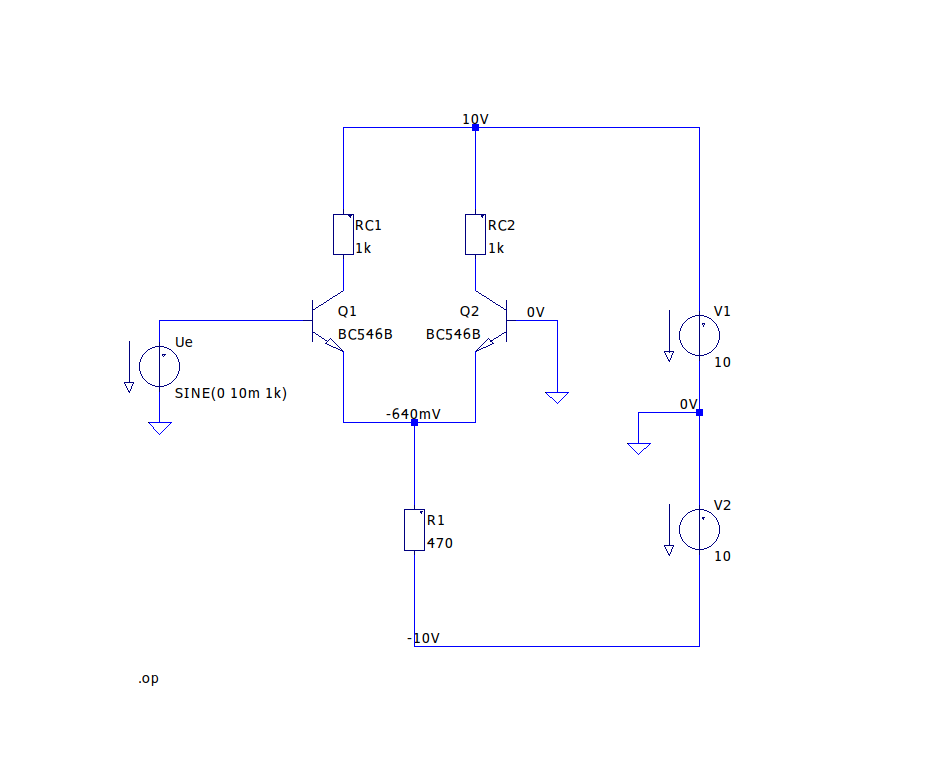
\includegraphics[scale=0.5]{../assets/images/EL2P1/DeepinScreenshot_select-area_20210417231020.png}
  \caption{Versuchsaufbau Wechselspannungsansteuerung}
\end{figure}

\subsection{Einfache Wechselspannungsansteuerung}

Wir stellen zunächst $U_e$ auf eine sinusförmige Wechselspannungsquelle mit einer Amplitude von $\hat{u} = 10mV$ und
einer Frequenz von $f = 1\mathrm{kHz}$ um. Darüberhinaus fügen wir nun noch zwei $R_C$-Widerstände in das Schaltbild
mit je $R_{C1,2} = \mathrm{1k}\Omega$ Betrachten wir nun die Kollektorspannung beider Transistoren, so erkennen wir, dass
beide Signale perfekt um 180° verschoben sind.

\begin{figure}[h]
  \centering
  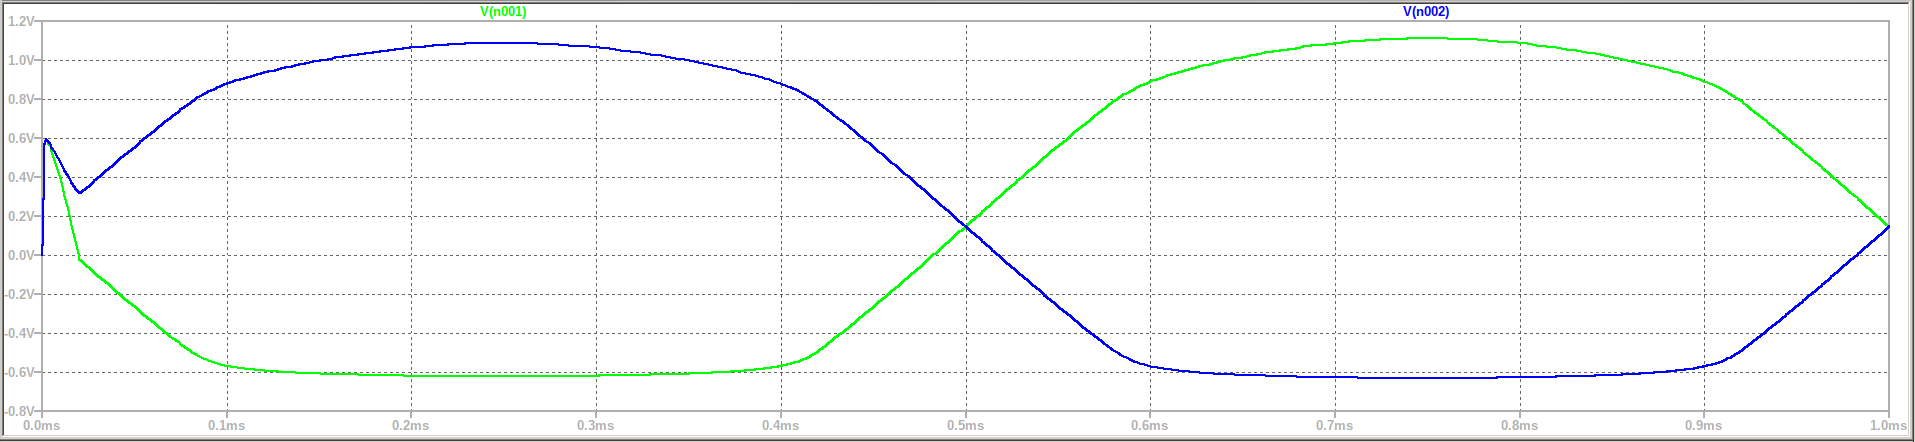
\includegraphics[scale=0.3]{../assets/images/EL2P1/DeepinScreenshot_select-area_20210417231348.png}
  \caption{Entstehendes Bild der einfachen Wechselspannungsansteuerung}
  \label{fig:diag2}
\end{figure}

\subsection{Doppelte Wechselspannungsansteuerung}

Wir verbinden nun die Basis des rechten Transistor nicht mehr mit GND sondern ebenfalls mit der Spannungsquelle
$U_e$. Wir passen dabei die Amplitude nun so an, dass beide Signale ähnliche Spitzenwerte erreichen wie bei Teilversuch 1.

\end{document}